\subsection{Book Extraction}
To extract the set of points that represented the book we used couple of thresholds in order to capture the book and reduce noise. First, we used the point cloud that can be seen in Figure \ref{fig:points} and subtracted the points belonging to the three planes. Now to eliminate other data points, such as outside the cabinate (see Figure \ref{fig:regionGrowing}), we subtracted all points that were to the left and right of the topmost plane, and ones that were below the corner point. Finally, to eliminate noise on the topmost plane, we extracted only the points that had the distance $\geq 1$ from the top plane. The result can be seen in Figure \ref{fig:bookPoints}.

\begin{figure}[H]
	\centering
	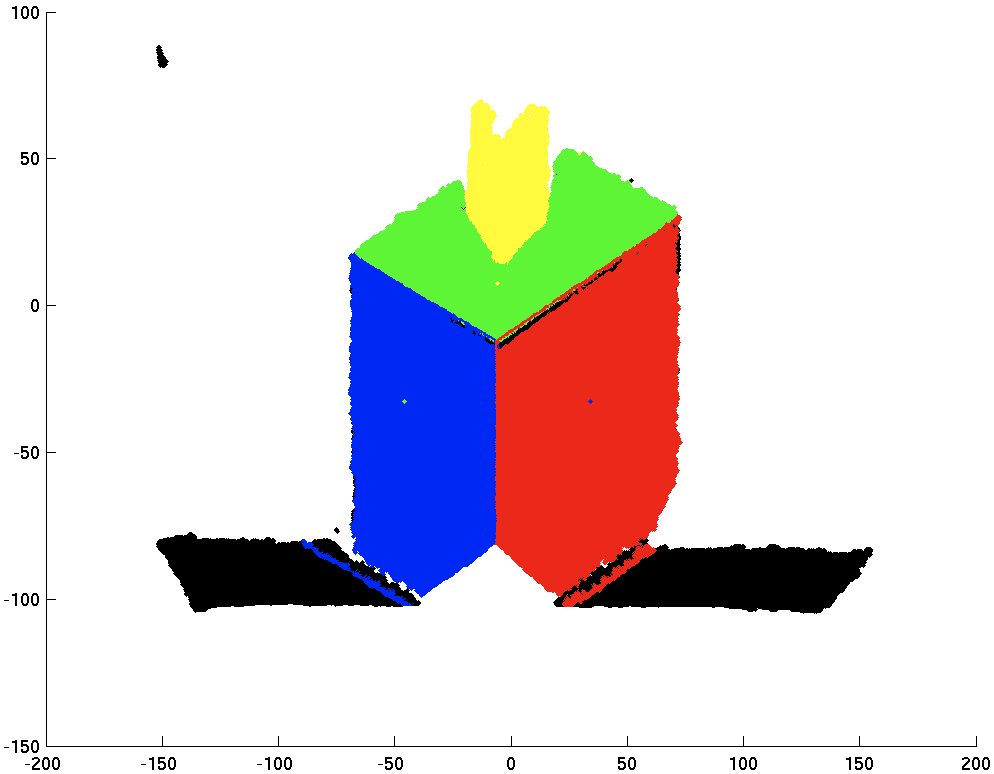
\includegraphics[width=0.5\textwidth]{Images/6-BookPoints(1).png}
	\label{fig:bookPoints}
	\caption{Book points extracted and displayed in yellow}
\end{figure}